\documentclass[addpoints,12pt]{exam}

\usepackage{amsmath}
\usepackage{amsthm}
\usepackage{graphicx}
\usepackage{enumitem}

\printanswers %Remove to hide answers
\pagestyle{headandfoot} %Adds Headers and Footers
\runningheadrule
\firstpageheader{Math 151}{Exam 1}{\today}
\runningheader{Math 151}
{Exam 1, Page \thepage\ of \numpages}
{\today}
\firstpagefooter{}{\thepage}{}
\runningfooter{}{\thepage}{}


\begin{document}

%The box at the top, and the name
\begin{center}
\fbox{\fbox{\parbox{5.5in}{\centering
Answer the questions in the spaces provided on the
question sheets. If you run out of room for an answer,
continue on the back of the page.}}}
\end{center}
\vspace{0.1in}
\makebox[\textwidth]{Name:\enspace\hrulefill}
\vspace{0.2in}

%Question Formatting
%\qformat{\textbf{Question \thequestion}\quad (\thepoints)\hfill}
%Point Table


%\begin{center}
%\gradetable[h][questions]
%\end{center}

%Beginning Questions
\begin{questions}
	\question Solve the following linear equation 
   \[
 2(x-1)+3 = x-3(x-1)~.
\]

 \begin{solution}

 \end{solution}
 
\question Solve the following equation 
   \[
 \frac{x}{5}- \frac{1}{2} = \frac{x}{6}~.
\]

\question The length of an American football field is 200 feet more than its width. If the perimeter is 1040 feet, then how wide is the field? 
\question You have 150 dollars to inverst. Part of the money is invested in an account through Yankton Financial paying $15\%$ annual interest. The rest of the money is to be invested in a second account at Vermillian Bank paying $13\%$ interest. If you would like $2\$$ a year in interest, how much should you invest into each account? Feel free to keep your answer unsimplified. 

\question Perform the following computation using complex numbers. 
   \[
		 (7+2i)-(5-7i)= 
\]



\question Perform the following computation using complex numbers. 
\[
		 (3+5i)(-5-i)=
\]

\question Solve the following quadratic equation by factoring~. 
\[
	x^{2}-3x-10=0 
\]

\question Solve the following quadratic equation by the square root property. 
   \[
5x^{2}+1=26
\]
\question Solve the following quadratic equation by completing the square 
   \[
x^{2}+6x-7=0
\]
\question Solve the following equation involving radicals~.
   \[
    \sqrt{2x-1}+2=x
	 \]

	 \question Solve the following equation involving rational exponents 
	    \[
	  7|x-3|+2=16
	 \]

\question Draw the number line for each of the four following intervals 
\begin{enumerate}

	\item $(1,6]$
	\item $[2,\infty)$
	\item $[-2,5]$
	\item $(-\infty,-2)$

\end{enumerate}

\question Solve the linear inequality
   \[
4(x+1)+2\geq 3x-13
\]

\question Solve the absolute value inequality 
\[
|3x-9| > 3
\]

\question Solve the system of linear equations

\begin{align*}
	x&+3y=8\\
	2x&-y=9\\
\end{align*}

\question Solve the system of linear equations 
\begin{align*}
	x&+2y=2 \\
		-4x&+3y = 25 \\
\end{align*}


\question Use the graph to evaluate the following function

\[
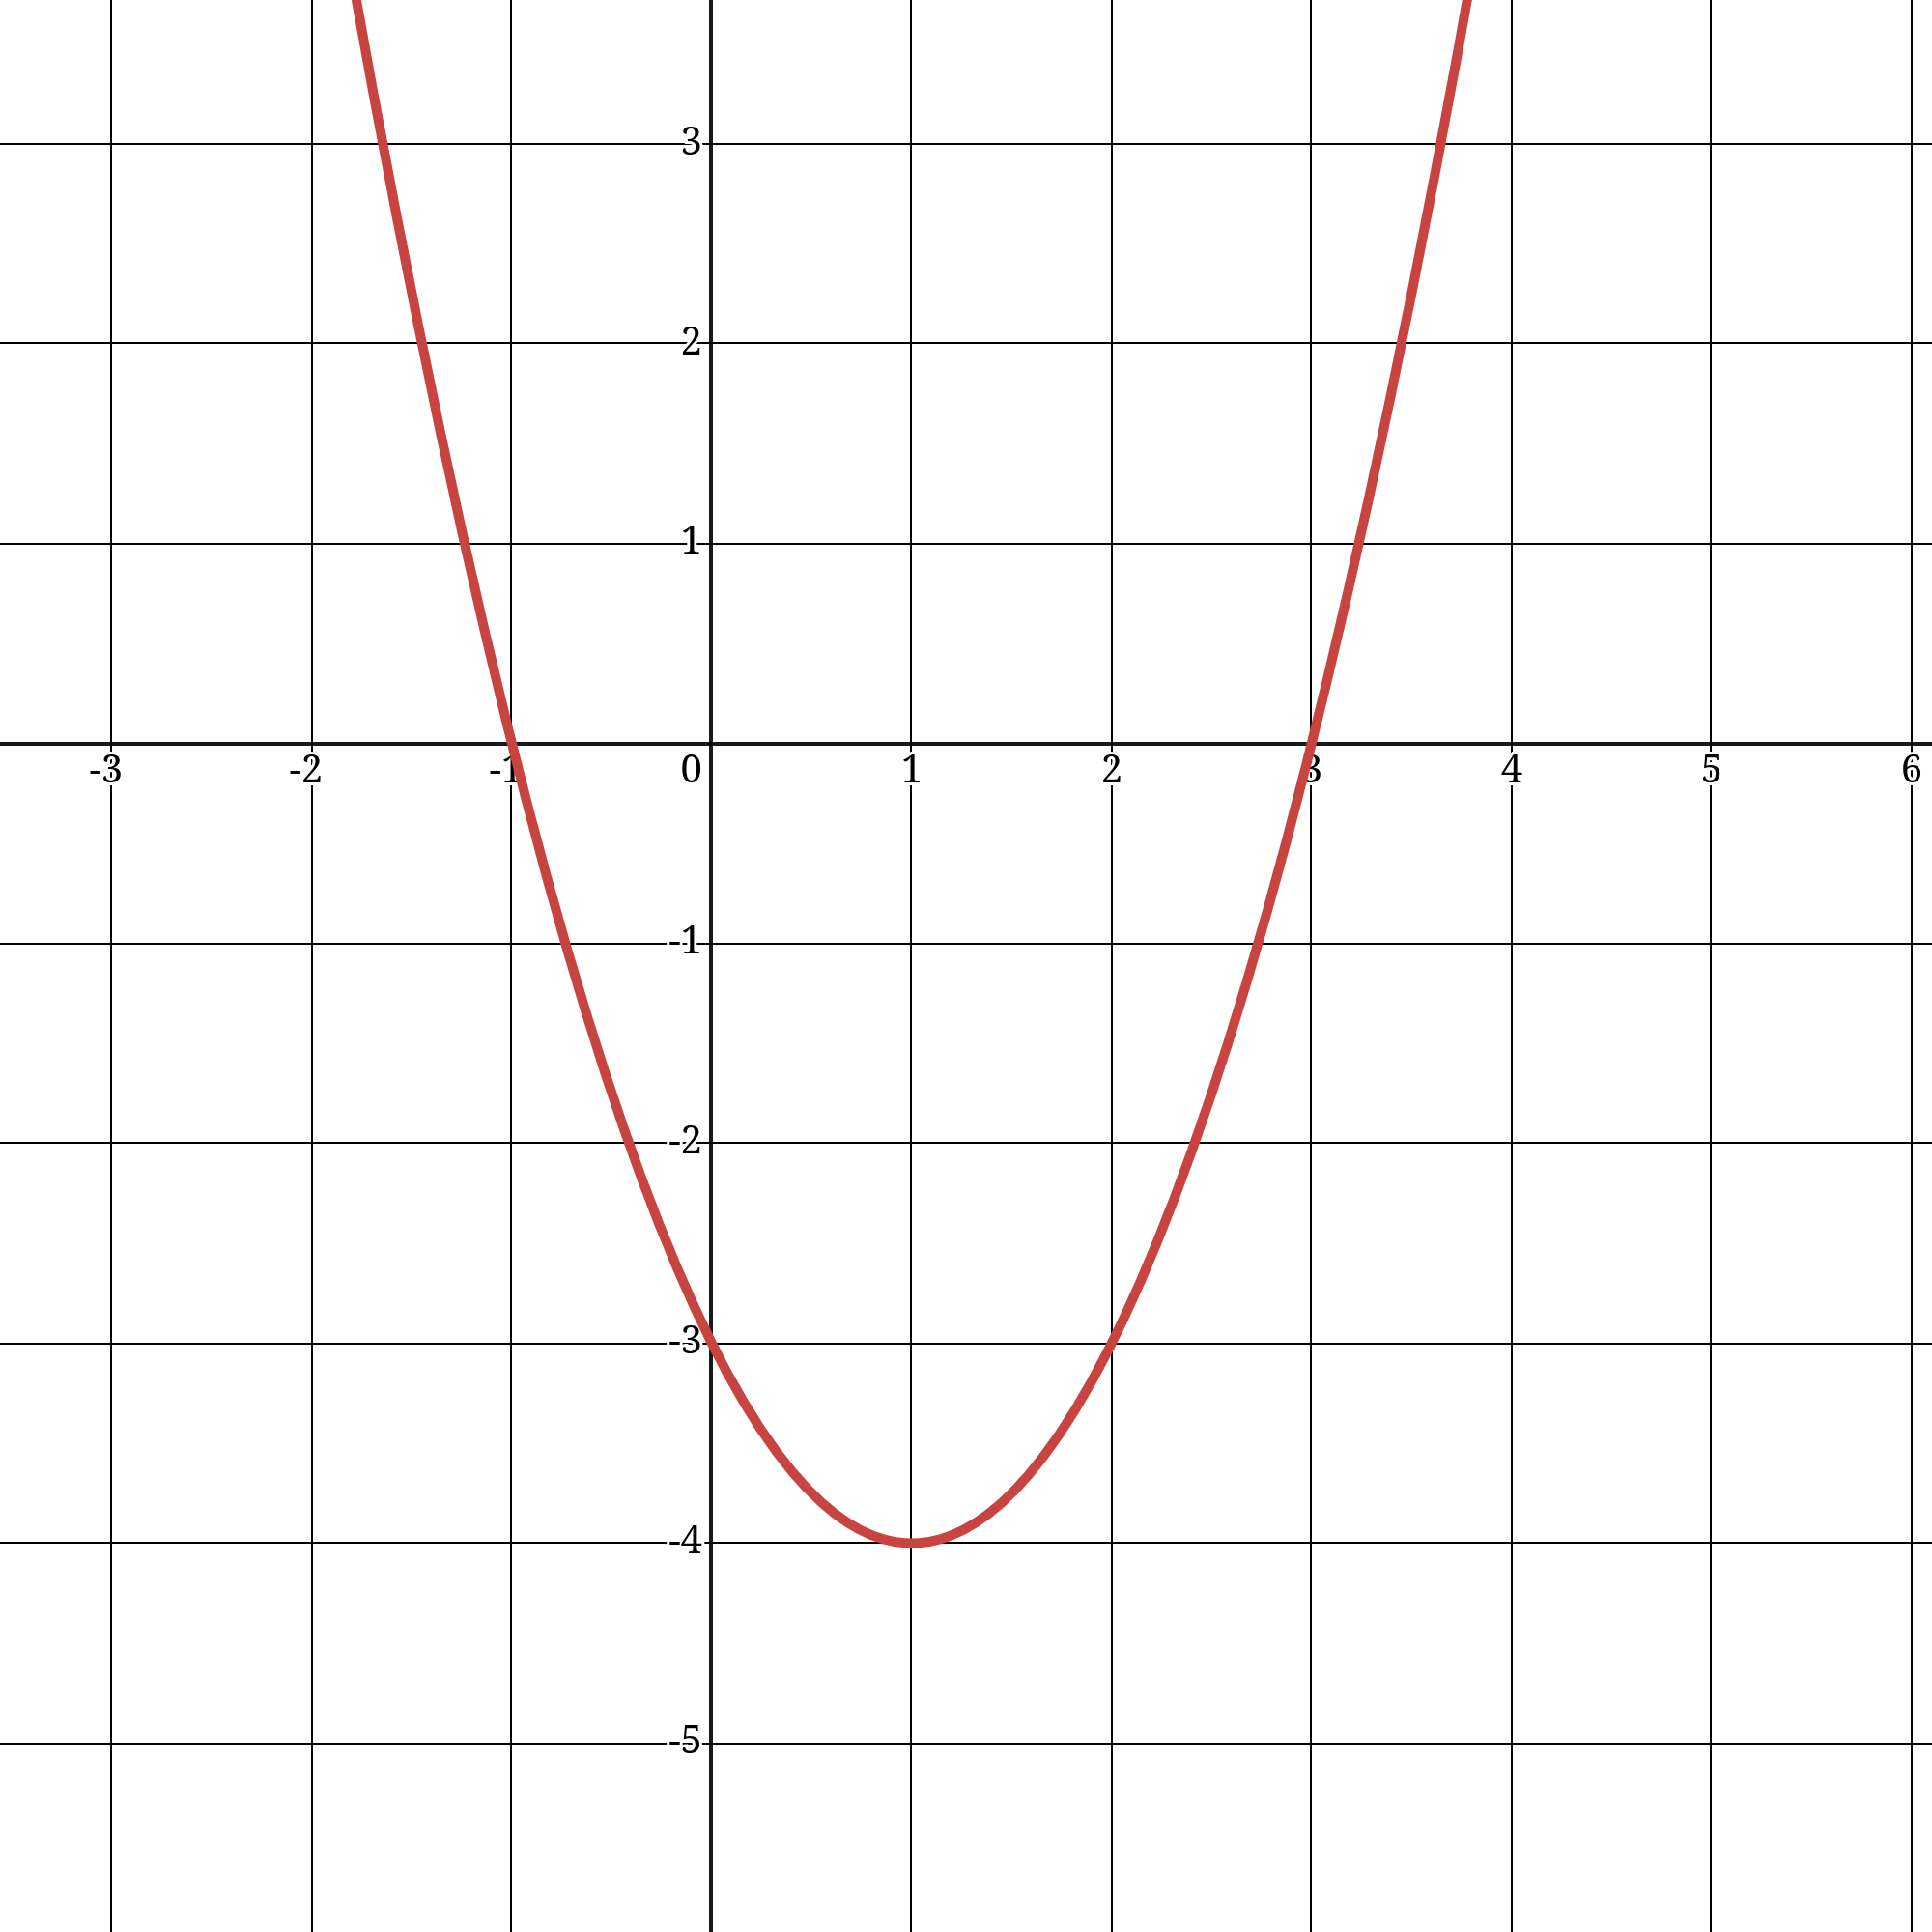
\includegraphics[scale = 0.1]{quadratic_graph}
\]

\question Evaluate the function
\[
f(x)=x^{2}+2x+3
\]
for the following function values 
\begin{enumerate}[label = \alph*)]
    \item $f(-2)=$ 
		\item $f(x+1)=$
		\item $f(-x)=$
\end{enumerate}

\question Find the relative maximum and minimums of the following graph 

\begin{figure}[htb!]
  \centering
  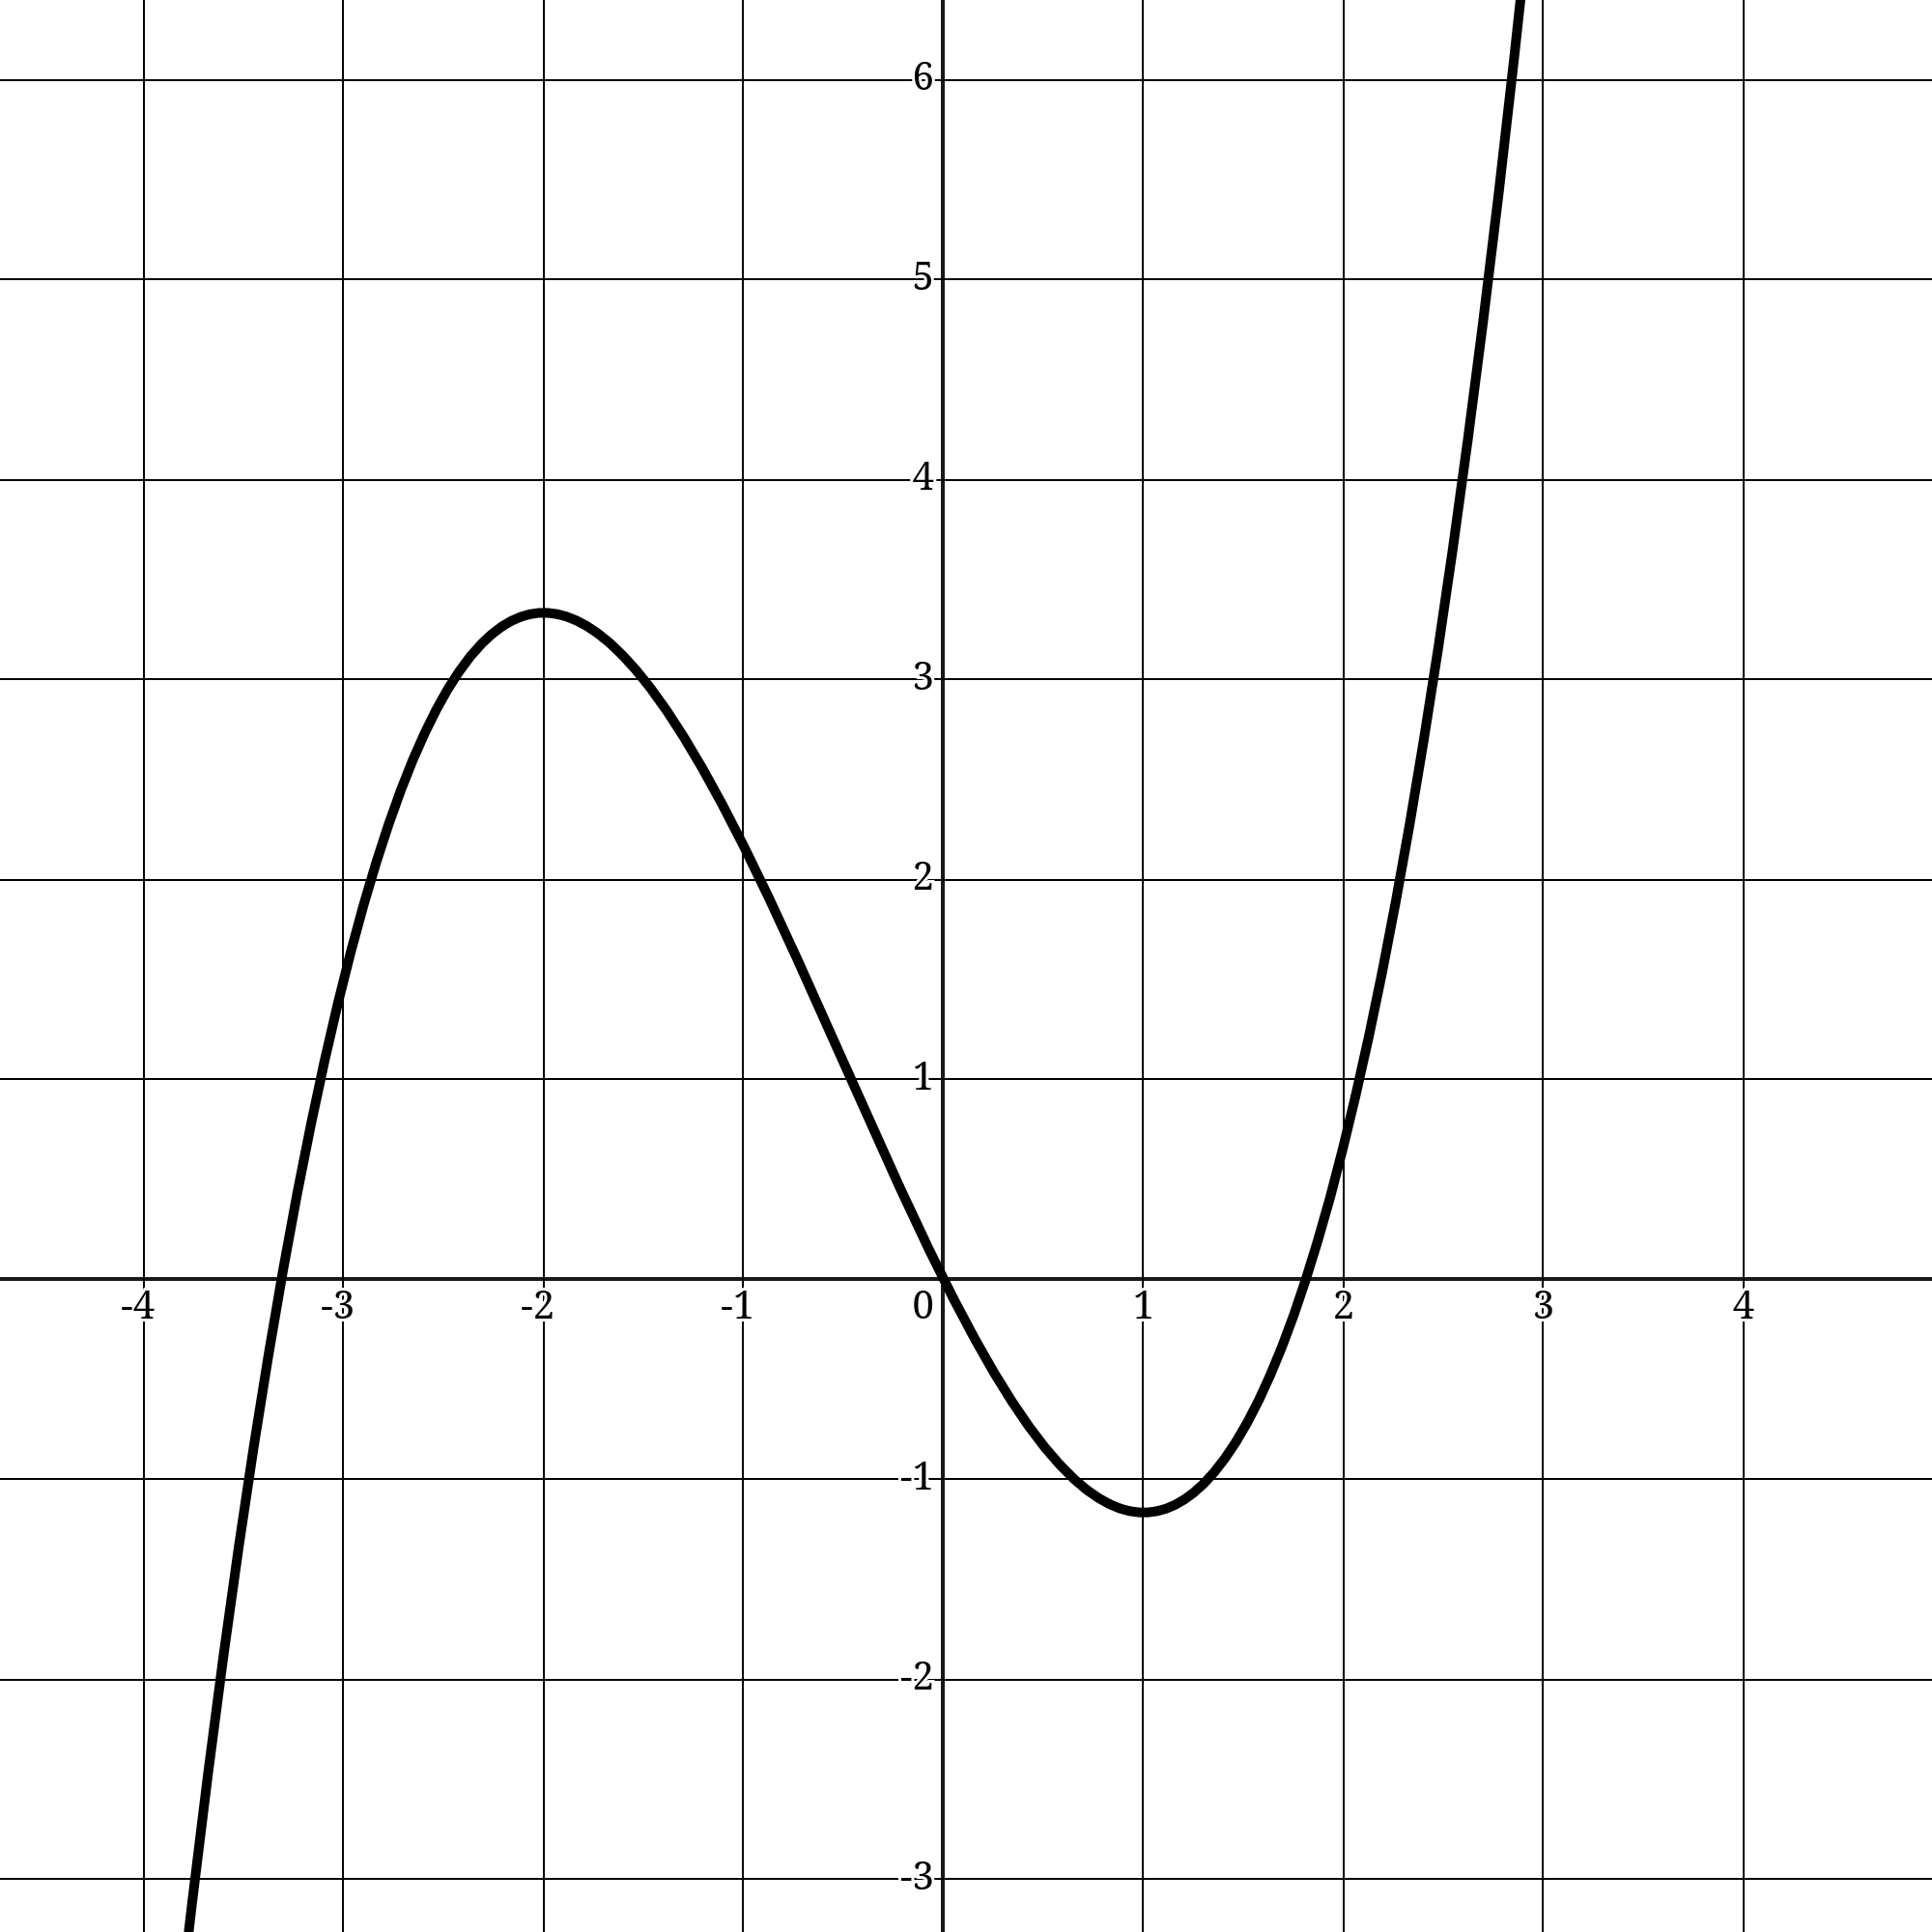
\includegraphics[scale = 0.1]{minmax}
\end{figure}

\question Give an example of an even function, and verify that it is an even function. 

\question Evaluate the following piecewise function at the following values
\[
	f(x) =
	\begin{cases}
   x+4 & x\leq -3 \\
	 -x+2 & x> -3 \\
	\end{cases}
\]

\begin{enumerate}
    \item $f(-5)=$
		\item $f(-3) = $
		\item $f(-1)= $
		\item $f(0)=$
\end{enumerate}

\end{questions}

\end{document}
